\section{The elephant walk and its crossing}\label{sec:erw}

In this section we reduce the elephant walk to a chain with a fixed first
step, prove that the crossing is unique, and find where it is. Throughout,
$n$ is even whenever $C_n$ appears, and $h=n/2$.

\begin{definition}[elephant walk]\label{def:erw}
Fix $0<\varepsilon<1$. Let $X_1$ be uniform on $\{\pm1\}$. For $t\ge1$ let
$U_t$ be uniform on $\{1,\dots,t\}$, and put $X_{t+1}=X_{U_t}$ with
probability $1-\varepsilon$ and $X_{t+1}=-X_{U_t}$ with probability
$\varepsilon$. All these choices are independent. We call the event
$X_{t+1}=-X_{U_t}$ a flip. As before, $A_n$ is the number of $i\le n$ with
$X_i=+1$, $C_n=\Prob(A_n=h)$ and $E_n=\Prob(A_n=n)$. The crossing
$\varepsilon_n$ is the value of $\varepsilon$ with $C_n=E_n$, and
$x_n=n\varepsilon_n$.
\end{definition}

In the notation of \cite{schutz2004} the memory parameter is
$p=1-\varepsilon$, and \cite{glrs2025} write $a=2p-1=1-2\varepsilon$. We
write $\Prob_+$ and $\E_+$ for the law and expectation given $X_1=+1$. Let
$M_t$ be the number of $i\le t$ with $X_i\ne X_1$, and put
$r_t(b)=\varepsilon+(1-2\varepsilon)b/t$ and $f_n(m)=\Prob_+(M_n=m)$.

\begin{lemma}\label{lem:erw-reduction}
The process $(M_t)_{t\ge1}$ is a Markov chain with $M_1=0$ and
$\Prob(M_{t+1}=b+1\mid M_t=b)=r_t(b)=1-\Prob(M_{t+1}=b\mid M_t=b)$, and it
is independent of $X_1$. For $0\le k\le n$,
$\Prob(A_n=k)=\frac12[f_n(n-k)+f_n(k)]$. In particular $C_n=f_n(h)$,
$E_n=\frac12(1-\varepsilon)^{n-1}$, and the law of $A_n$ is symmetric about
$h$.
\end{lemma}

\begin{proof}
Given $X_1,\dots,X_t$, the copied step $X_{U_t}$ differs from $X_1$ with
probability $M_t/t$. So $X_{t+1}\ne X_1$ with conditional probability
$(1-\varepsilon)M_t/t+\varepsilon(1-M_t/t)=r_t(M_t)$. This depends only on
$M_t$ and not on $X_1$, which proves the first claim. On $\{X_1=+1\}$ we
have $A_n=n-M_n$, and on $\{X_1=-1\}$ we have $A_n=M_n$. Averaging over
$X_1$ gives the formula for $\Prob(A_n=k)$, which does not change under
$k\mapsto n-k$. Finally $M_n\le n-1$, so $f_n(n)=0$, and
$f_n(0)=\prod_{t=1}^{n-1}(1-r_t(0))=(1-\varepsilon)^{n-1}$.
\end{proof}

\begin{remark}\label{rem:families}
For $\varepsilon\le\frac12$ we can write
$r_t(b)=(1-2\varepsilon)\frac bt+2\varepsilon\cdot\frac12$. So each new
step copies a uniformly chosen earlier step exactly with probability
$1-2\varepsilon$, and it is a fresh fair sign with probability
$2\varepsilon$. The steps then split into clusters, each made of a fresh
sign and every step copied from it directly or through other copies, and
the cluster signs are i.i.d.\ and fair. These are the clusters of
Bernoulli bond percolation with retention parameter $1-2\varepsilon$ on a
random recursive tree \cite{kursten2016}. We do not use this remark in the
proofs.
\end{remark}

\begin{proposition}\label{prop:mlr}
For every $n\ge2$ and $1\le k\le n-1$, the ratio $f_n(k)/f_n(0)$ is
strictly increasing in $\varepsilon\in(0,1)$. Hence $\Prob(A_n=k)/E_n$ is
strictly increasing in $\varepsilon$ for every $1\le k\le n-1$. In
particular $C_n/E_n$ is strictly increasing, the crossing $\varepsilon_n$
exists and is unique, and $\varepsilon_n<\frac12$. In fact $C_n\ge2E_n$ for
$\varepsilon\ge\frac12$.
\end{proposition}

Divide the probability of every path of $M$ by the probability of the path
that never flips. Then each step contributes a factor that only grows with
$\varepsilon$.

\begin{proof}
The probability of a path of $M$ is a product of $n-1$ factors, namely
$r_s(b_s)$ for an up step at time $s$ and $1-r_s(b_s)$ otherwise, where
$b_s$ is the state at time $s$. We divide it by
$f_n(0)=(1-\varepsilon)^{n-1}$. With $y=b_s/s\in[0,1)$ the factors
become
\[
 \frac{r_s(b_s)}{1-\varepsilon}=\frac{\varepsilon+(1-2\varepsilon)y}{1-\varepsilon}
 \qquad\text{and}\qquad
 \frac{1-r_s(b_s)}{1-\varepsilon}=1-y\,\frac{1-2\varepsilon}{1-\varepsilon},
\]
with derivatives $(1-y)/(1-\varepsilon)^2>0$ and
$y/(1-\varepsilon)^2\ge0$ in $\varepsilon$. Both factors are positive, since
$r_s(b_s)=\varepsilon(1-y)+(1-\varepsilon)y$ lies strictly between 0
and 1. So the ratio for each path is nondecreasing in $\varepsilon$, and it
is strictly increasing if the path has an up step. Summing over the paths
with $k\ge1$ up steps proves the first claim. The second follows, since
$\Prob(A_n=k)/E_n=[f_n(n-k)+f_n(k)]/f_n(0)$ by
Lemma~\ref{lem:erw-reduction}. As $\varepsilon\to0$ we have $C_n\to0$ and
$E_n\to\frac12$. For $\varepsilon\ge\frac12$ every $r_s(b)$ lies in
$[1-\varepsilon,\varepsilon]$, so each path of $M$ that ends at $h$ has
probability at least $(1-\varepsilon)^{n-1}=2E_n$. Hence $C_n\ge2E_n$. The
ratio $C_n/E_n$ is continuous and strictly increasing, so it equals 1 at
exactly one $\varepsilon$, and this $\varepsilon$ lies in $(0,\frac12)$.
\end{proof}

Next we look at the first flip. For $1\le s\le n$ let
$V_s(b)=\Prob_+(M_n=h\mid M_s=b)$. For $1\le t\le h$ let
\[
 \pi_t=\frac{t\prod_{i=1}^{t-1}(h-i)}{\prod_{i=1}^{t}(n-i)},\qquad
 c_1=\sum_{t=1}^h\pi_t,\qquad w_t=\frac{\pi_t}{c_1},
\]
so that $(w_t)_{1\le t\le h}$ is a probability vector.

\begin{proposition}\label{prop:first-mutation}
Let $n\ge2$ be even.
\begin{enumerate}[(a)]
\item $C_n=\sum_{t=1}^h\varepsilon(1-\varepsilon)^{t-1}V_{t+1}(1)$.
\item $C_n$ is a polynomial in $\varepsilon$ with $C_n(0)=0$. At
$\varepsilon=0$ we have $V_{t+1}(1)=\pi_t$, and
$C_n'(0)=c_1=\frac4{n+2}$ exactly.
\item For each fixed $t$, $w_t\to t2^{-t-1}$ as $n\to\infty$. For every even
$n$, $\sum_tw_tt=3-\frac6{h+2}$ and $\sum_tw_t(t+1)^3\le124$.
\end{enumerate}
\end{proposition}

\begin{proof}
(a) Under $\Prob_+$ the first flip happens at step $t+1$ exactly when
$M_s=0$ for $s\le t$ and $M_{t+1}=1$. Since $r_s(0)=\varepsilon$, this has
probability $(1-\varepsilon)^{t-1}\varepsilon$, and by the Markov property
the chain then ends at $h$ with probability $V_{t+1}(1)$. At time $t+1$
there are $t$ steps equal to $X_1$, and this number never decreases. So
$V_{t+1}(1)=0$ for $t>h$. Paths with no flip end at $0\ne h$. Since
$C_n=f_n(h)$, this proves (a).

(b) Every transition probability is affine in $\varepsilon$, so $C_n$ and
$V_{t+1}(1)$ are polynomials in $\varepsilon$. By (a), $C_n(0)=0$ and
$C_n'(0)=\sum_tV_{t+1}(1)|_{\varepsilon=0}$. At $\varepsilon=0$ we have
$r_s(b)=b/s$, so $M$ is P\'olya's urn. At time $t+1$ it holds $t$ balls of
one color and 1 of the other, and it makes $n-t-1$ more draws. By the
Beta-binomial law of P\'olya's urn, $h-1$ of these draws are of the
minority color with probability
$\binom{n-t-1}{h-1}\mathrm B(h,h)/\mathrm B(1,t)=t\binom{n-t-1}{h-1}(h-1)!^2/(n-1)!$,
which equals $\pi_t$. The Chu--Vandermonde identity
$\sum_t\binom t1\binom{n-1-t}{h-1}=\binom n{h+1}$ then gives
$c_1=\binom n{h+1}(h-1)!^2/(n-1)!=n/(h(h+1))=4/(n+2)$.

(c) Write $\pi_t=\frac t{n-t}\prod_{i=1}^{t-1}\frac{h-i}{n-i}$. For fixed
$t$ each fraction $\frac{h-i}{n-i}$ tends to $\frac12$, so
$n\pi_t\to t2^{1-t}$. Since $nc_1\to4$, we get $w_t\to t2^{-t-1}$. For the
moments, $w_t$ is proportional to $\binom t1\binom{n-1-t}{h-1}$, and
Chu--Vandermonde gives $\sum_t\binom tj\binom{n-1-t}{h-1}=\binom n{h+j}$.
Since $t^2=\binom t1+2\binom t2$, we get
$\sum_tw_tt=1+2\binom n{h+2}/\binom n{h+1}=1+\frac{2(h-1)}{h+2}=3-\frac6{h+2}$.
Similarly $t(t+1)^3=8\binom t1+38\binom t2+54\binom t3+24\binom t4$, and
$\binom n{h+j}\le\binom n{h+1}$ for $j\ge1$. So
$\sum_tw_t(t+1)^3\le8+38+54+24=124$.
\end{proof}

To first order in $\varepsilon$ the walk flips once, and after that it is
P\'olya's urn. If the flip comes at step $t+1$, the urn starts with $t$
balls of one color and 1 of the other, and $\pi_t$ is the chance that it
ends with $h$ of each. For large $n$ the minority fraction is close to a
Beta$(1,t)$ variable, whose density at $\frac12$ is $t2^{1-t}$. Summing
$t2^{1-t}$ over $t$ gives the 4 in $c_1\approx4/n$.

To go beyond first order we follow the path after the first flip. For
$1\le t\le h$ we write $\E^{\br}_t$ for the expectation over paths from
$M_{t+1}=1$ to $M_n=h$ whose $h-1$ up steps are placed uniformly at random
among the $n-t-1$ remaining steps. This is P\'olya's urn from state
$(t+1,1)$ conditioned to end at $h$ (Lemma~\ref{lem:A-polya}). For
$1\le b\le u-1$ let
\[
 \theta_u(b)=\frac{n(u-2b)^2}{2(n-u)b(u-b)},\qquad
 A_t=\sum_{u=t+1}^{n-1}\E^{\br}_t\,\theta_u(M_u).
\]
The second-order bridge sum $B_t\ge0$ is defined in
Proposition~\ref{prop:A-bridge}, and the lower bound $J_n$ in
\eqref{eq:A-Jn}. We also put $\kappa=2\varepsilon/(1-4\varepsilon)$,
$H_k=\sum_{j\le k}1/j$ and
$\mathcal G(t)=(t+11)\bigl(\log\frac{(t+1)^2}{4t}+\frac23\bigr)-H_t+\frac2{3t}$.

\begin{theorem}\label{thm:erw-bounds}
Let $n\ge2$ be even.
\begin{enumerate}[(a)]
\item For $0<\varepsilon<\frac14$,
\[
 C_n\le U_n:=\varepsilon c_1e^{\kappa H_{n-1}}\sum_{t=1}^hw_t(1-\varepsilon)^{t-1}e^{\kappa\mathcal G(t)}.
\]
\item For $0<\varepsilon\le\frac12$ and $1\le t\le h$,
$\log V_{t+1}(1)\ge\log\pi_t+\varepsilon A_t-\varepsilon^2B_t$. Hence
$C_n\ge J_n$.
\item For even $n\ge64$ and $0<\varepsilon\le\frac1{100(1+\log n)}$,
\[
 -11\varepsilon-\varepsilon^2(84\log n+1.05\cdot10^5)
 \le\log C_n-\log\frac{4\varepsilon}{n+2}-2\varepsilon\log n\le566\varepsilon .
\]
In particular
$\bigl|\log C_n-\log\frac{4\varepsilon}{n+2}-2\varepsilon\log n\bigr|\le566\varepsilon$
there.
\end{enumerate}
\end{theorem}

\begin{proof}
Parts (a) and (b) follow from Propositions~\ref{prop:A-super}
and~\ref{prop:A-bridge} together with
Proposition~\ref{prop:first-mutation}(a). Part (c) is proved in
Appendix~\ref{app:erw}.
\end{proof}

The constants in (c) are crude. By Theorem~\ref{thm:K2}, the coefficient of
$\varepsilon$ in $\log(C_n/(c_1\varepsilon))$ is $2\log n+K_2+o(1)$ with
$K_2\approx-1.54$. At the crossing the bounds (a) and (b) are close to
$C_n$ (Table~\ref{tab:erw-crossing}). The exception is
$U_{50}/C_{50}=69.5$, since the upper bound needs $\kappa\log n$ to be
small.

After the first flip the chain $M$ at time $s$ is P\'olya's urn with
$\beta s$ extra balls of each color, where $\beta=\varepsilon/(1-2\varepsilon)$
(Lemma~\ref{lem:A-polya}). These extra balls pull the minority fraction
toward $\frac12$, and along a path that ends at the center the pull adds
about $2\varepsilon/s$ to the log-probability at time $s$. Summing over
$s\le n$ gives the factor $n^{2\varepsilon}$ in (c).

We now locate the crossing. By Theorem~\ref{thm:erw-bounds}(c),
$C_n\approx4x/n^2$ when $\varepsilon=x/n$ and $x$ is of order $\log n$.
Also $E_n=\frac12(1-x/n)^{n-1}\approx\frac12e^{-x}$. Setting them equal
gives $x+\log x\approx2\log n-\log8$. So let $L_n=2\log n-\log8$ and
$G(x)=x+\log x$, and let $g_n$ be the root of $G(g_n)=L_n$.

\begin{theorem}\label{thm:erw-crossing}
As $n\to\infty$ over even $n$, the following hold.
\begin{enumerate}[(a)]
\item $x_n+\log x_n=L_n-\eta_n$ with
$\eta_n=\dfrac{2x_n\log n+x_n^2/2}{n}+O\Bigl(\dfrac{\log n}n\Bigr)$. So
$0<g_n-x_n=O((\log n)^2/n)$ for large $n$.
\item $x_n=g_n-\dfrac{2g_n\log n+g_n^2/2}{n(1+1/g_n)}+O\Bigl(\dfrac{\log n}{n}\Bigr)$.
\item $x_n=2\log n-\log\log n-\log16+O\Bigl(\dfrac{\log\log n}{\log n}\Bigr)$.
\end{enumerate}
\end{theorem}

\begin{proof}
(a) Put $F(x)=\log C_n(x/n)-\log E_n(x/n)$ for $0<x<n$. By
Proposition~\ref{prop:mlr}, $F$ is strictly increasing and $x_n$ is its
only zero. Let $n\ge6\cdot10^4$ and $1\le x\le2L_n$. Then $x\le4\log n$
and $400\log n(1+\log n)\le n$, so $\varepsilon=x/n\le\frac1{100(1+\log n)}$
and Theorem~\ref{thm:erw-bounds}(c) applies. For $0\le y\le\frac12$ we have
$-y-\frac{y^2}2-y^3\le\log(1-y)\le-y-\frac{y^2}2$. We use this with
$y=x/n$ in $E_n=\frac12(1-y)^{n-1}$, together with
$0\le\log(1+\frac2n)\le\frac2n$ and $x^2\le2n$. Then
\[
 F(x)=G(x)-L_n+\frac{2x\log n-x+x^2/2}{n}+R_n(x),\qquad
 |R_n(x)|\le\frac{570x+3}{n}.
\]
Hence $|F(x)-G(x)+L_n|\le\rho_n$ on $[1,2L_n]$, where
$\rho_n=(2L_n(2\log n+L_n+571)+3)/n=O((\log n)^2/n)$. Since $G'\ge1$ and
$G(g_n)=L_n$, this gives $F(x)<0$ for $1\le x<g_n-\rho_n$ and $F(x)>0$ for
$g_n+\rho_n<x\le2L_n$. As $L_n-\log L_n\le g_n\le L_n$, for large $n$ both
ranges are nonempty, and so $|x_n-g_n|\le\rho_n$. In particular
$x_n\to\infty$. Now $F(x_n)=0$ gives $G(x_n)=L_n-\eta_n$ with
$\eta_n=(2x_n\log n+x_n^2/2)/n-x_n/n+R_n(x_n)$, and the last 2 terms are at
most $(571x_n+3)/n=O(\log n/n)$ in absolute value. This is (a), except for
the sign. Since $x_n\to\infty$, the term $2x_n\log n/n$ is larger than
$(571x_n+3)/n$ for large $n$. Then $\eta_n>0$, so $G(x_n)<G(g_n)$ and
$x_n<g_n$.

(b) By the mean value theorem, $x_n-g_n=-\eta_n/G'(\xi)$ for some $\xi$
between $x_n$ and $g_n$. Here $G'(\xi)=1+1/\xi=1+1/g_n+O(1/n)$, since
$|\xi-g_n|=O((\log n)^2/n)$ and $g_n\ge\log n$ for large $n$. As
$\eta_n=O((\log n)^2/n)$, we get
$x_n-g_n=-\eta_n/(1+1/g_n)+O((\log n)^2/n^2)$. Replacing $x_n$ by $g_n$ in
the main term of $\eta_n$ changes it by $O((\log n)^3/n^2)$. This gives
(b).

(c) Since $g_n=L_n-\log g_n$ and $L_n-\log L_n\le g_n\le L_n$, we have
$\log g_n=\log L_n+O(\log L_n/L_n)$. Also
$\log L_n=\log2+\log\log n+O(1/\log n)$. So
$g_n=2\log n-\log\log n-\log16+O(\log\log n/\log n)$, and
$x_n-g_n=O((\log n)^2/n)$ by (a).
\end{proof}

The $O$-constants in (a) and (b) are explicit once $n\ge6\cdot10^4$, but we
have not turned them into an explicit $n$ beyond which $g_n>x_n$.
Table~\ref{tab:erw-crossing} gives exact crossings on the grid
$n=50\cdot2^k$, computed from the recursion for $f_n$ in
Lemma~\ref{lem:erw-reduction} (Section~\ref{sec:verify}). The second-order
formula (b) is already within $0.07$ of $x_n$ at $n=400$. On the other hand
$x_n/\log n$ is only $1.55$ at $n=51200$, so the limit 2 in (c) is
approached slowly.

\begin{table}[t]
\centering\small
\begin{tabular}{@{}rllllllr@{}}
\toprule
$n$ & $x_n$ & $g_n$ & $x_n-x_{\mathrm{2nd}}$ & $x_n/\log n$ & $J_n/C_n$ & $U_n/C_n$ & $D(n)$\\
\midrule
50 & 3.9404868665 & 4.288636 & $+0.3452$ & 1.007 & 0.915 & 69.5 & $-0.02123$\\
400 & 7.6292168962 & 7.843768 & $+0.0621$ & 1.273 & 0.9905 & 1.770 & $-0.03319$\\
1600 & 10.2405649147 & 10.340051 & $+0.0179$ & 1.388 & 0.99868 & 1.188 & $+0.02921$\\
3200 & 11.5468344808 & 11.610464 & $+0.0097$ & 1.431 & 0.99954 & 1.0996 & $+0.04786$\\
12800 & 14.1588452626 & 14.182921 & $+0.0028$ & 1.497 & 0.99995 & 1.0289 & $+0.06416$\\
51200 & 16.7784677365 & 16.786946 & $+0.0008$ & 1.547 & n/c & n/c & $+0.06522$\\
\bottomrule
\end{tabular}
\caption{Exact crossings of the elephant walk (to 10 decimal places), the
root $g_n$ of $G(g)=L_n$, the error of the second-order formula, the
explicit bounds of Theorem~\ref{thm:erw-bounds} at the crossing, and the
difference $D(n)$ of Theorem~\ref{thm:erw-markov}. Here $x_{\mathrm{2nd}}$
is the formula of Theorem~\ref{thm:erw-crossing}(b) without its error term.
The tabulated $J_n$ keeps only the terms $t\le60$ of \eqref{eq:A-Jn}, so it
is still a lower bound for $C_n$. The entries marked n/c were not
computed.}
\label{tab:erw-crossing}
\end{table}

Now we compare with the Markov walk. Paper~A \cite{paperA} shows that
$z=z_n$ solves $z+\frac12\log z=\log n+\frac12\log\frac\pi8+o(1)$. Doubling
gives $2z+\log(2z)=2\log n+\log\frac\pi4+o(1)$, which has the same form as
the equation for $x_n$ in Theorem~\ref{thm:erw-crossing}. The right sides
differ by $\log(2\pi)$.

\begin{theorem}\label{thm:erw-markov}
Let $p_n$ be the central crossing of the Markov walk with $n$ steps in
\cite{paperA}, and let $z_n=n(1-p_n)$. As $n\to\infty$ over even $n$,
\[
 D(n):=x_n-\bigl(2z_n-\log(2\pi)\bigr)=\frac{c_*}{\log n}
 +O\Bigl(\frac{(\log\log n)^2}{(\log n)^2}\Bigr),\qquad
 c_*=\tfrac12\log(2\pi)-\tfrac14=0.668939\ldots
\]
\end{theorem}

\begin{proof}
Write $L=\log n$ and $c_0=\frac12\log\frac\pi8$. The third-order expansion
in the uniform Bessel approximation theorem of \cite{paperA} says that
\[
 z_n=L+d+\frac eL+O\Bigl(\frac{(\log L)^2}{L^2}\Bigr),\qquad
 d=-\tfrac12\log L+c_0,\quad e=\tfrac14\log L-\tfrac12c_0+\tfrac18.
\]
Then $\log z_n=\log L+d/L+O((\log L)^2/L^2)$. Since $e+d/2=\frac18$, we
get $z_n+\frac12\log z_n=L+c_0+\frac1{8L}+O((\log L)^2/L^2)$. Put $Y=2z_n$
and $\ell=\log(2\pi)$. Since $2c_0+\log2=\log\frac\pi4$, this gives
$Y+\log Y=2L+\log\frac\pi4+\frac1{4L}+O((\log L)^2/L^2)$. Also
$Y=2L-\log L+O(1)$, so $\log(1-\ell/Y)=-\ell/(2L)+O(\log L/L^2)$. Using
$\log\frac\pi4-\ell=-\log8$, we get
\[
 G(Y-\ell)=Y+\log Y-\ell+\log\Bigl(1-\frac\ell Y\Bigr)
 =L_n+\frac1{4L}-\frac\ell{2L}+O\Bigl(\frac{(\log L)^2}{L^2}\Bigr)
 =L_n-\frac{c_*}L+O\Bigl(\frac{(\log L)^2}{L^2}\Bigr).
\]
By Theorem~\ref{thm:erw-crossing}(a), $G(x_n)=L_n-\eta_n$ with
$\eta_n=O(L^2/n)$. Both $x_n$ and $Y-\ell$ are $2L+O(\log L)$, so
$G'=1+O(1/L)$ between them. The mean value theorem then gives
$x_n-(Y-\ell)=c_*/L+O((\log L)^2/L^2)+O(L^2/n)$, and the last term is
absorbed. Since $Y-\ell=2z_n-\log(2\pi)$, this is the claim.
\end{proof}

We computed $z_n$ from the exact law of the Markov walk \cite{paperA}. The
difference $D(n)$ is negative up to $n=400$ and changes sign near $n=800$.
At $n=3200$, $12800$ and $51200$ it is $0.0479$, $0.0642$ and $0.0652$,
against $c_*/\log n=0.083$, $0.071$ and $0.062$. So the asymptotic regime
is reached slowly (Figure~\ref{fig:crossing}).

\begin{figure}[t]
\centering
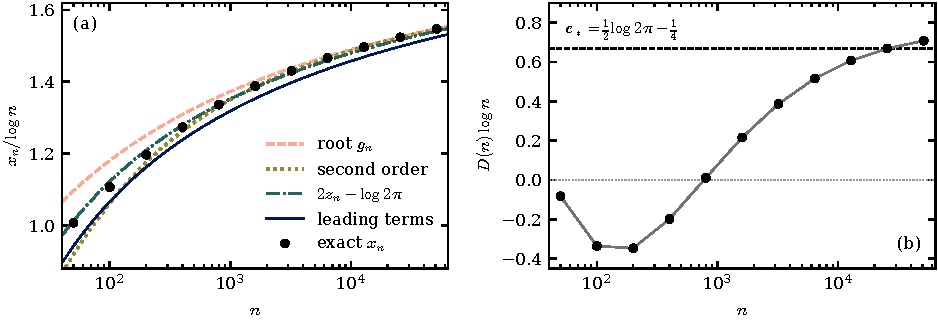
\includegraphics{figures/crossing}
\caption{(a) The scaled elephant crossing $x_n/\log n$. The dots are the
exact roots for $n=50\cdot2^k$. The curves are the root $g_n$ of
$x+\log x=2\log n-\log8$, the second-order formula of
Theorem~\ref{thm:erw-crossing}(b) without its error term, the Markov
crossing through $2z_n-\log(2\pi)$, and the leading terms
$2\log n-\log\log n-\log16$ of Theorem~\ref{thm:erw-crossing}(c). (b) The
difference $D(n)=x_n-(2z_n-\log(2\pi))$ of Theorem~\ref{thm:erw-markov}
times $\log n$. By that theorem it tends to $c_*$ (dashed), with an error
of order $(\log\log n)^2/\log n$, so the approach is slow.}
\label{fig:crossing}
\end{figure}

Theorem~\ref{thm:erw-bounds}(c) does not identify the $O(\varepsilon)$
term. For small $\varepsilon$ we can find it exactly. Write
$C_n=c_1\varepsilon+c_2\varepsilon^2+O(\varepsilon^3)$ as $\varepsilon\to0$
(Proposition~\ref{prop:first-mutation}(b)) and put $k_2(n)=c_2/c_1$. As in
Section~\ref{sec:intro}, $\gamma$ is Euler's constant.

\begin{theorem}\label{thm:K2}
\begin{enumerate}[(a)]
\item For every even $n\ge2$, $k_2(n)=\sum_{t=1}^hw_t\bigl[A_t-(t-1)\bigr]$.
\item For each fixed $t\ge1$, as $n\to\infty$ over even $n$,
$A_t-2\log n\to A^\infty_t:=2(\gamma-1-\log2)+(t-2)H_{t-1}$.
\item As $n\to\infty$ over even $n$,
\[
 k_2(n)-2\log n\to K_2:=\sum_{t\ge1}t2^{-t-1}\bigl[A^\infty_t-(t-1)\bigr]
 =2\gamma-2-\log2=-1.5387158508\ldots
\]
\end{enumerate}
\end{theorem}

\begin{proof}
Part (a) follows from Proposition~\ref{prop:first-mutation}(a) by
differentiating the bridge formula of Proposition~\ref{prop:A-bridge} at
$\varepsilon=0$. Parts (b) and (c) are
proved in Appendix~\ref{app:erw}.
\end{proof}

From the Taylor coefficients of $C_n$ we get $k_2(n)-2\log n=-1.585878$,
$-1.546572$ and $-1.541005$ at $n=1600$, $12800$ and $51200$. So,
informally,
$C_n\approx\frac{4\varepsilon}{n+2}n^{2\varepsilon}e^{K_2\varepsilon}$
when $\varepsilon\log n$ is small.

\begin{remark}\label{rem:refined}
Let $\hat x_n$ solve
\[
 \log\frac{4x}{n(n+2)}+\frac xn\,k_2(n)=\log\frac12+(n-1)\log\Bigl(1-\frac xn\Bigr).
\]
The lower bound behind Theorem~\ref{thm:erw-bounds} gives
$x_n\le\hat x_n+O((\log n)^3/n^2)$, and we prove this at the end of
Appendix~\ref{app:erw}. A matching upper bound would need
$\log C_n\le\log(\varepsilon c_1)+\varepsilon k_2(n)+O(\varepsilon^2(\log n)^k)$
for some $k$, which we do not have. The rest of this remark is numerical
only. Let $k_3(n)$ be the coefficient of $\varepsilon^2$ in
$\log(C_n/(c_1\varepsilon))$, computed from the Taylor coefficients of
$C_n$. It lies between $-8.8$ and $-8.7$ for $12800\le n\le51200$. If we
add $\frac{x^2}{n^2}k_3(n)$ to the left side of the equation, the root
differs from $x_n$ by $5.3\cdot10^{-7}$ at $n=3200$ and by
$3.6\cdot10^{-10}$ at $n=51200$. We predicted $x_{51200}$ in this way
before computing it.
\end{remark}
